\documentclass[a4paper,12pt]{article}

\usepackage{indentfirst}
\usepackage[utf8]{inputenc}
\usepackage{graphicx}
\usepackage{float}
\usepackage[portuguese]{algorithm2e}
\usepackage{amsmath}

\title{Um Exemplo de Artigo em \LaTeX}
\author{Tiago Luiz Schmitz\\UDESC
        \and 
        JUCA\\Universidade de exemplos}
\date{\today}


\begin{document}

\maketitle

\begin{abstract}
\noindent Isto é um resumo do artigo.\\
Síntese (2 ou 3 parágrafos) com a ideia principal do artigo.
\end{abstract}


\section{Introdução}

\section{Background}
\subsection{Conceitos básicos em XXX}
\subsubsection{Conceitos básicos em XXX.1}
Aqui vai um exemplo de uma lista numerada
\begin{enumerate}
\item primeira característica desta fase
\item segunda característica desta fase
\item terceira característica desta fase
\end{enumerate}

Aqui vai um exemplo de uma lista não-numerada
\begin{itemize}
\item primeira característica desta fase
\item segunda característica desta fase
\item terceira característica desta fase
\end{itemize}

\subsubsection{Conceitos básicos em XXX.2}
Seguem-se algumas definições fundamentais para se perceberem as ideias 
defendidas a seguir:
\begin{description}
\item[conceito 1] respectiva definição 1
\item[conceito 2] descrição do  conceito 2
\end{description}


\subsection{Conceitos básicos em YYY}
A tabela \ref{tab1} compara dois softwares.
	\begin{table}[H]
	      \begin{tabular}{| l |c |r |}
	      \hline
	        Software & função 1 & função 2 \\
	        \hline
	        Jucas Corp. & X &  \\
	        Gueno Corp. & X & X \\
	        \hline
	      \end{tabular}
	      \caption{Comparação de dois softwares}
	      \label{tab1}
	\end{table}

              
\section{A Proposta}
A figura \ref{fig1} representa uma comparação entre trabalho do tipógrafo e o latex
       \begin{figure}[H]
                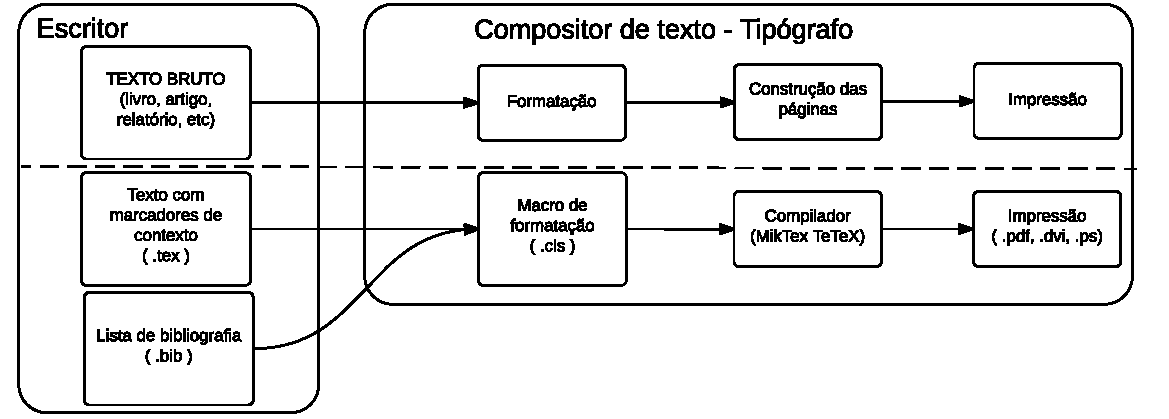
\includegraphics[scale=0.63]{img/tipografovslatex.pdf}    
                \caption{tipográfo X Latex}
                \label{fig1}     
             \end{figure} 

\section{A sua Implementação}


\begin{algorithm}[H]
 \KwData{Esse texto}
 \KwResult{Como ler um artigo}
 Inicialização\;
 \While{não for o final do documento}{
  Leia atual\;
  \eIf{Entendido}{
   Vá para a próxima seção\;
   A próxima seção torna-se a atual\;
   }{
   Volte para o inicio da seção atual\;
  }
 }
 \caption{Como ler um artigo}
 \label{alg1}
\end{algorithm}
\section{Avaliação}
A equação (\ref{for1})  apresenta uma integral de 0 a $\infty$.
\begin{align}
	\label{for1}	\int_0^\infty e^{-x^2} dx=\frac{\sqrt{\pi}}{2}
\end{align}

\section{Conclusão}
Síntese do que foi dito.\\
Lista dos resultados atingidos:
\begin{itemize}
\item resultado 1
\item resultado 2 e teste de bibliografia \cite{Bulfinch1998}
\end{itemize}
Conclusão final e Trabalho Futuro.

\bibliographystyle{plain}
\bibliography{n2library.bib}

\end{document}
